\section{Functional Architecture}

\subsection{Introduction}

\begin{frame}
\frametitle{Functional Architecture}
The functional architecture is initially developed during the research phase
and refined as development matures to production.

\begin{itemize}
    \item The main components of a system are identified
    \item Specific algorithms which realize the components are developed
    \item High-level interfaces between components are created
\end{itemize}

\begin{block}{}
The functional architecture for an autonomous driving vehicle has evolved
over the past decade and is converging towards an industry standard.
\end{block}
\end{frame}

\begin{frame}
\frametitle{Sense - Plan - Act}
\framesubtitle{Common Autonomous Vehicle Functional Architecture}
The \emph{Sense - Plan - Act} architecture is still predominant in modern autonomous
vehicle architectures.

\vspace{1cm}

\begin{center}
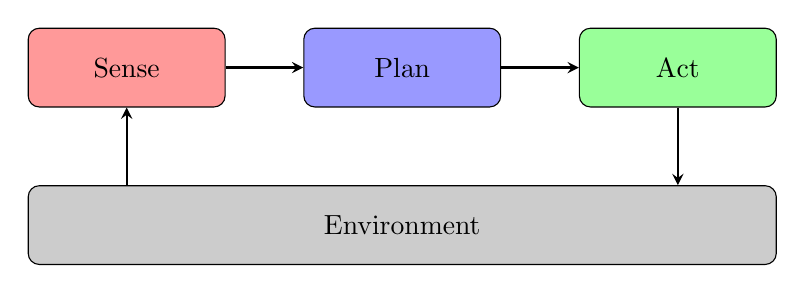
\begin{tikzpicture}[node distance=3.5cm]
    \node (sense)[rectangle,rounded corners,minimum width=2.5cm,minimum height=1cm,text centered,draw=black,fill=red!40]{Sense};
    \node (plan)[right of=sense,rectangle,rounded corners,minimum width=2.5cm,minimum height=1cm,text centered,draw=black,fill=blue!40]{Plan};
    \node (act)[right of=plan,rectangle,rounded corners,minimum width=2.5cm,minimum height=1cm,text centered,draw=black,fill=green!40]{Act};
    \node (environment)[below of=plan,yshift=1.5cm,rectangle,rounded corners,minimum width=9.5cm,minimum height=1cm,text centered,draw=black,fill=gray!40]{Environment};
    \draw [thick,->,>=stealth] (sense) -- (plan);
    \draw [thick,->,>=stealth] (plan) -- (act);
    \draw [thick,->,>=stealth] (act) -- ([xshift=3.5cm]environment.north);
    \draw [thick,<-,>=stealth] (sense) -- ([xshift=-3.5cm]environment.north);
    \end{tikzpicture}
\end{center}
\end{frame}

\begin{frame}
\frametitle{Sense - Plan - Act}
\framesubtitle{Common Autonomous Vehicle Functional Architecture}
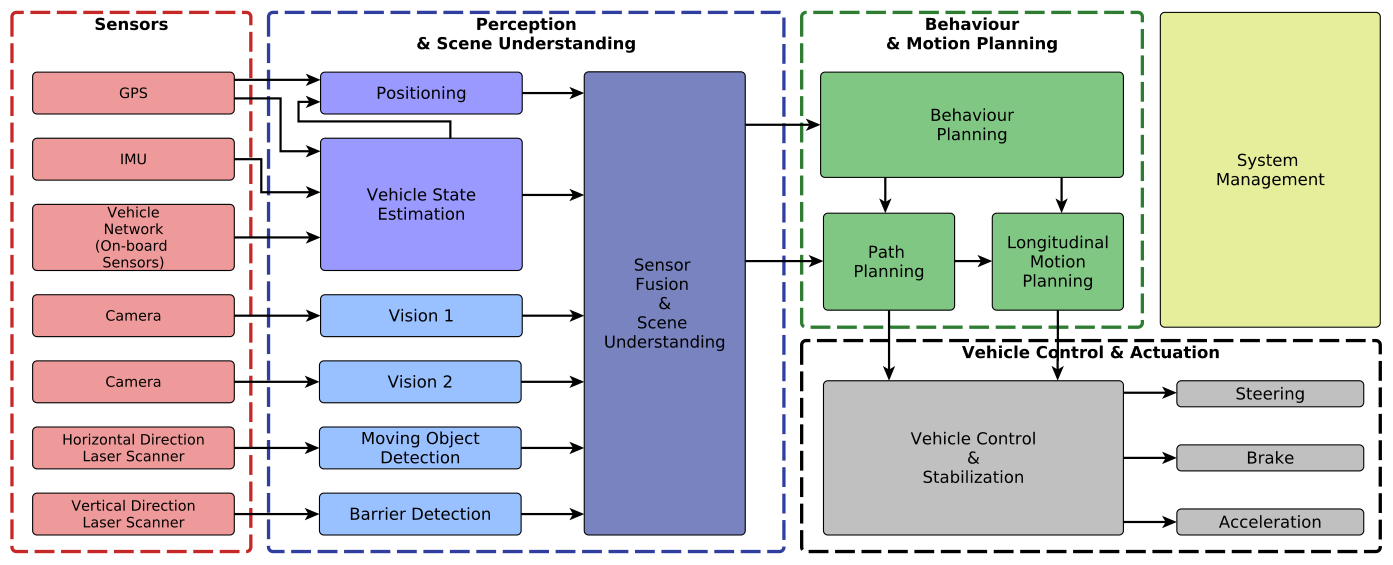
\includegraphics[width=\textwidth]{images/tas_2016_fig4_av_functional_architecture.png}
\tiny{Architecture image from \cite{Tas2016-sd} based on the vehicle that won the
Korean Autonomous Vehicle Competition \cite{Jo2014-na}}.
\end{frame}

\subsection{Sensors}

\begin{frame}
\frametitle{Sensors}
Autonomous vehicles use a combination of cameras, radar and lidar sensors to
sense and perceive the environment. \\
\vspace{0.25cm}
\centering
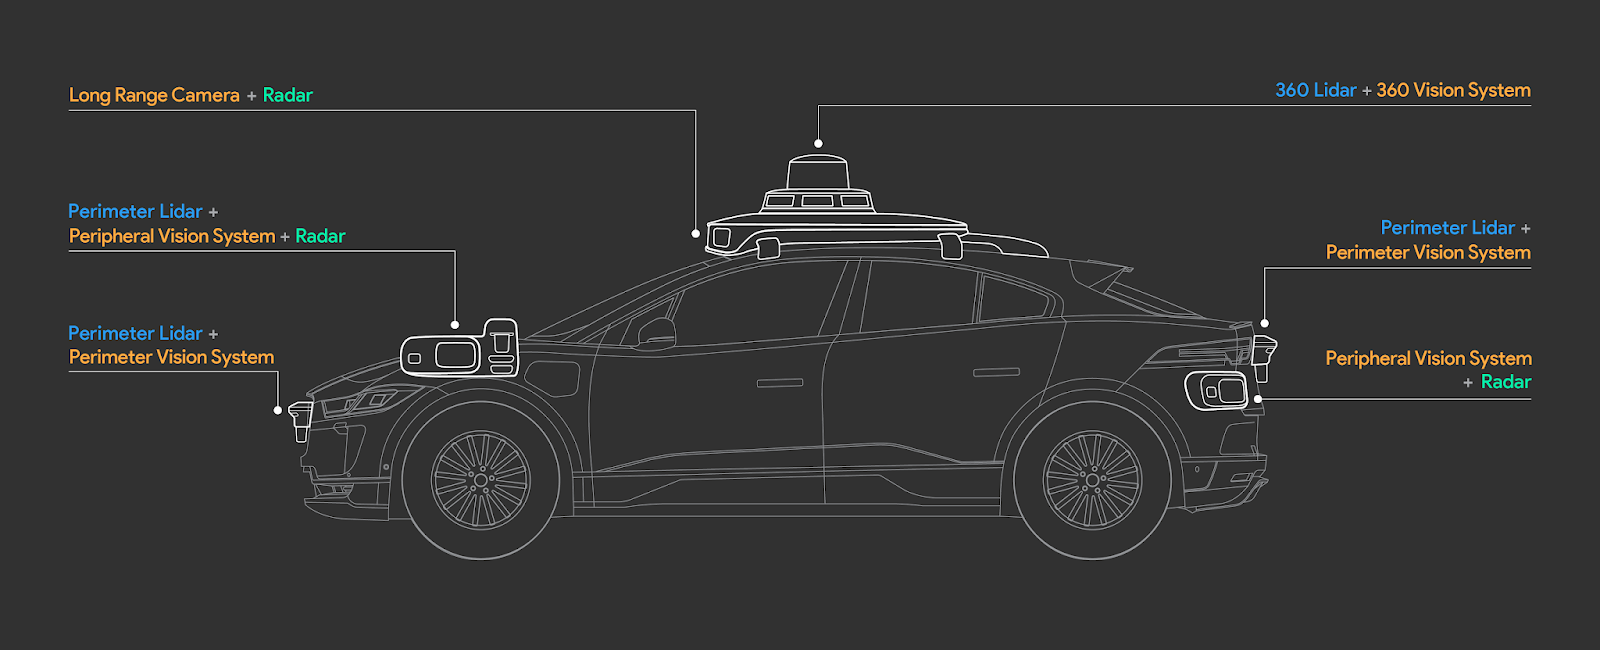
\includegraphics[width=0.9\textwidth]{images/waymo_sensors.png}\\
\footnotesize{Waymo sensor suite\footnotemark[1]}
\footnotetext[1]{\tiny{\url{https://blog.waymo.com/2020/03/introducing-5th-generation-waymo-driver.html}}}
\end{frame}

\begin{frame}
\frametitle{Sensors}
\framesubtitle{Camera}
\begin{columns}[T]
    \begin{column}{.5\textwidth}
        \centering
        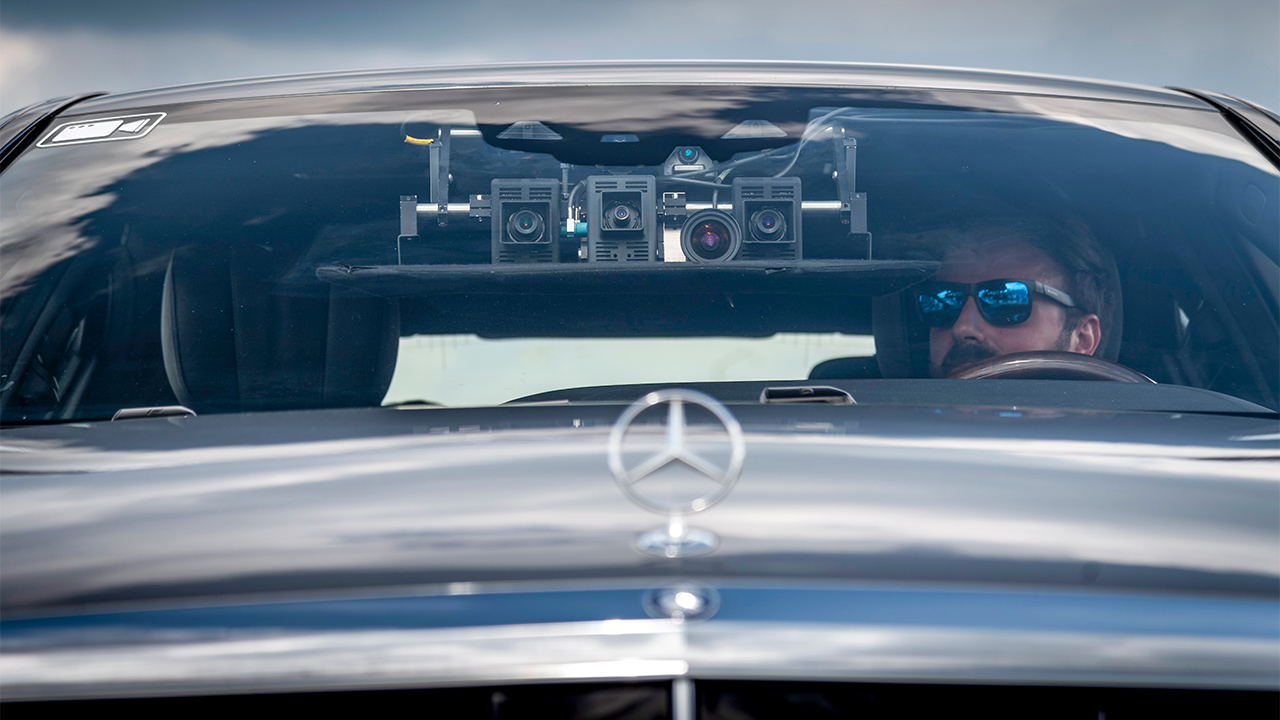
\includegraphics[width=0.6\textwidth]{images/daimler_cameras.jpg}\\
        \tiny{Source: Daimler\footnotemark[1]}\\
        \vspace{0.3cm}
        \href{https://www.youtube.com/watch?v=rACZACXgreQ}{
        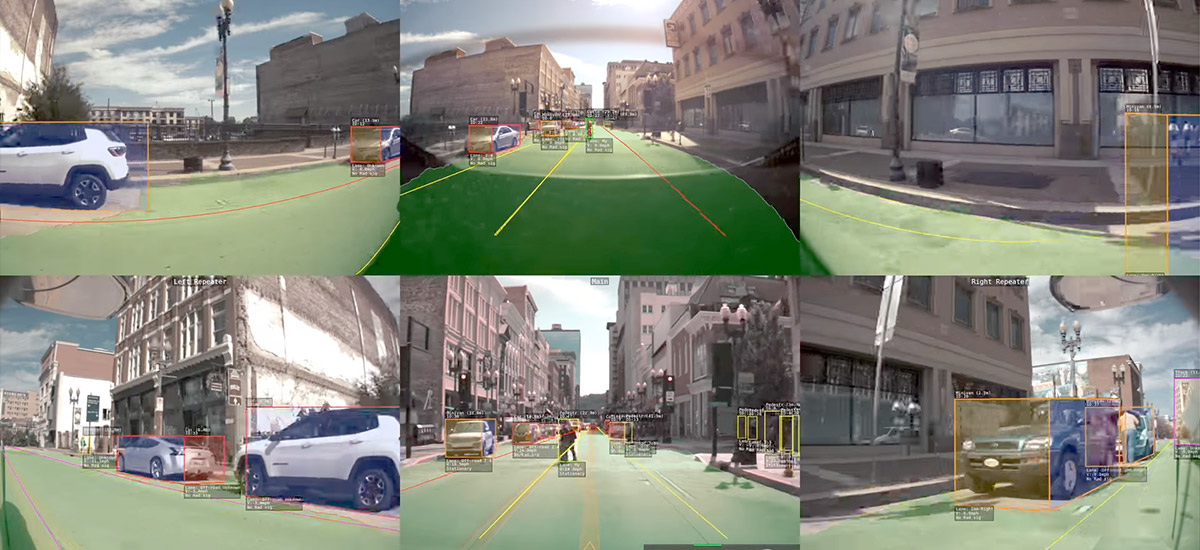
\includegraphics[width=0.9\textwidth]{images/tesla_autopilot_cameras.jpg}}\\
        \tiny{Tesla camera system, Source: YouTube (greentheonly)\footnotemark[2]}
    \end{column}
    \begin{column}{.5\textwidth}
        \footnotesize
        Vision sensors are the basis for an autonomous driving system, providing
        important perception input for many different purposes.
        \vspace{0.25cm}
        \begin{columns}[T]
            \begin{column}{0.45\textwidth}
                \footnotesize
                Capabilities:
                \begin{itemize}
                    \item Dynamic object detection
                    \item Static object detection
                    \item Lane and road detection
                    \item Classification
                    \item Traffic sign/light detection
                \end{itemize}
            \end{column}
            \begin{column}{0.55\textwidth}
                \footnotesize
                Important properties:
                \begin{itemize}
                    \item High dynamic range
                    \item $360\deg$ field of view
                    \item Global shutter
                    \item Low cost
                    \item No distance or velocity measurements
                \end{itemize}
            \end{column}
        \end{columns}
    \end{column}
\end{columns}

\footnotetext[1]{\tiny{\url{https://www.daimler.com/magazine/technology-innovation/automation-daimler-immendingen-camera-radar-lidar.html}}}
\footnotetext[2]{\tiny{\url{https://www.youtube.com/watch?v=rACZACXgreQ}}}
\end{frame}

\begin{frame}
\frametitle{Sensors}
\framesubtitle{Radar}
\begin{columns}[T]
    \begin{column}{.4\textwidth}
        \centering
        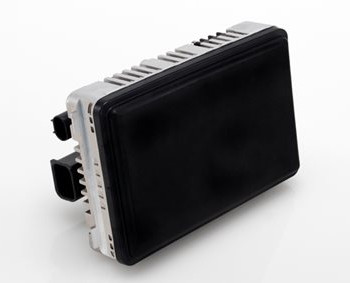
\includegraphics[width=0.3\textwidth]{images/continental_radar.jpg}\\
        \vspace{0.1cm}
        \tiny{Source: Continental\footnotemark[1]}\\
        \vspace{0.3cm}
        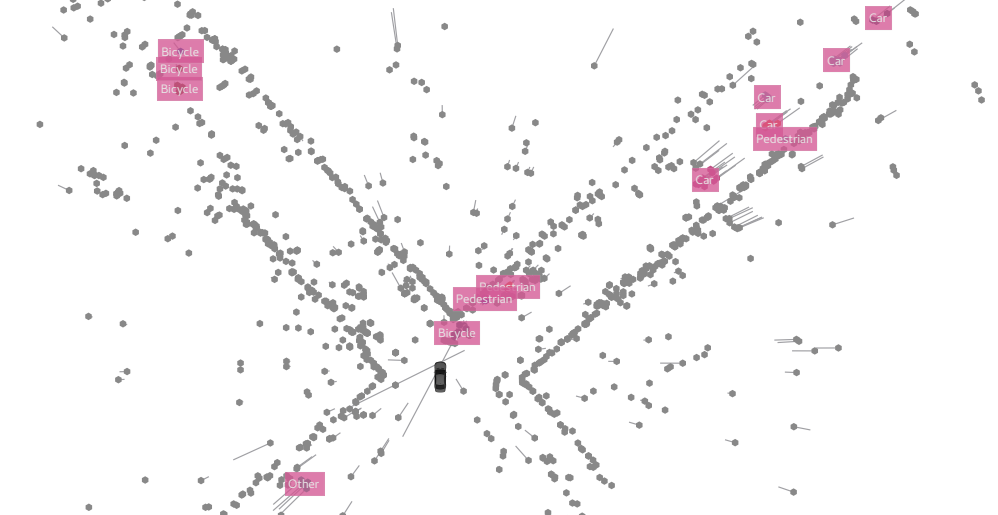
\includegraphics[width=\textwidth]{images/daimler_radar_dataset.png}\\
        \tiny{Source: Daimler, RadarScenes dataset\footnotemark[2]}
    \end{column}
    \begin{column}{.6\textwidth}
        \footnotesize
        Radar has been the workhorse of ADAS for over two decades, being the main
        sensor for ACC and continues its importance in autonomous driving systems.
        \vspace{0.2cm}
        \begin{columns}[T]
            \begin{column}{0.4\textwidth}
                \footnotesize
                Capabilities:
                \begin{itemize}
                    \item Dynamic object detection
                    \item Static object detection
                    \item Road boundary detection
                \end{itemize}
            \end{column}
            \begin{column}{0.6\textwidth}
                \footnotesize
                Important properties:
                \begin{itemize}
                    \item Robust in weather, e.g. rain, fog, etc.
                    \item Direct measurement of speed
                    \item Reasonable cost
                    \item Low resolution, poor vertical separation
                \end{itemize}
            \end{column}
        \end{columns}
    \end{column}
\end{columns}
\footnotetext[1]{\tiny{\url{https://www.continental-automotive.com/en-gl/Passenger-Cars/Autonomous-Mobility/Enablers/Radars/Long-Range-Radar/ARS540}}}
\footnotetext[2]{\tiny{\url{https://radar-scenes.com/}}}
\end{frame}

\begin{frame}
\frametitle{Sensors}
\framesubtitle{Lidar}
\begin{columns}[T]
    \begin{column}{.5\textwidth}
        \centering
        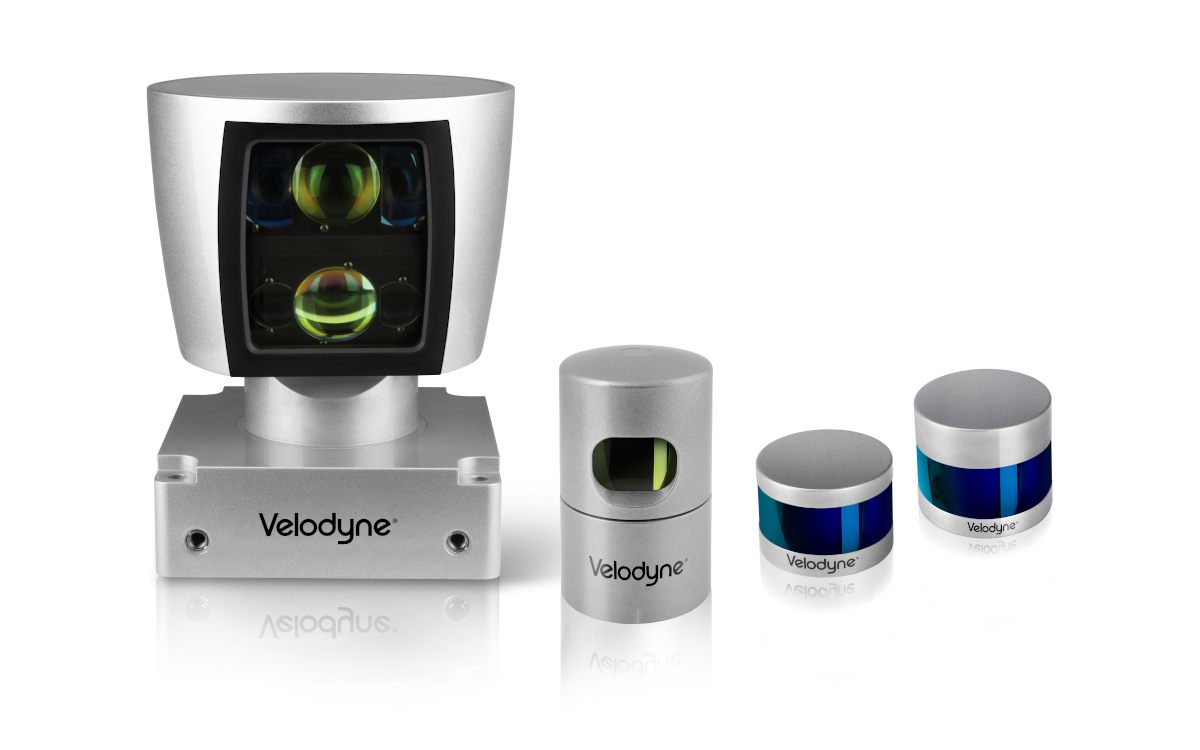
\includegraphics[width=0.5\textwidth]{images/velodyne_lidars.png}\\
        \vspace{0.2cm}
        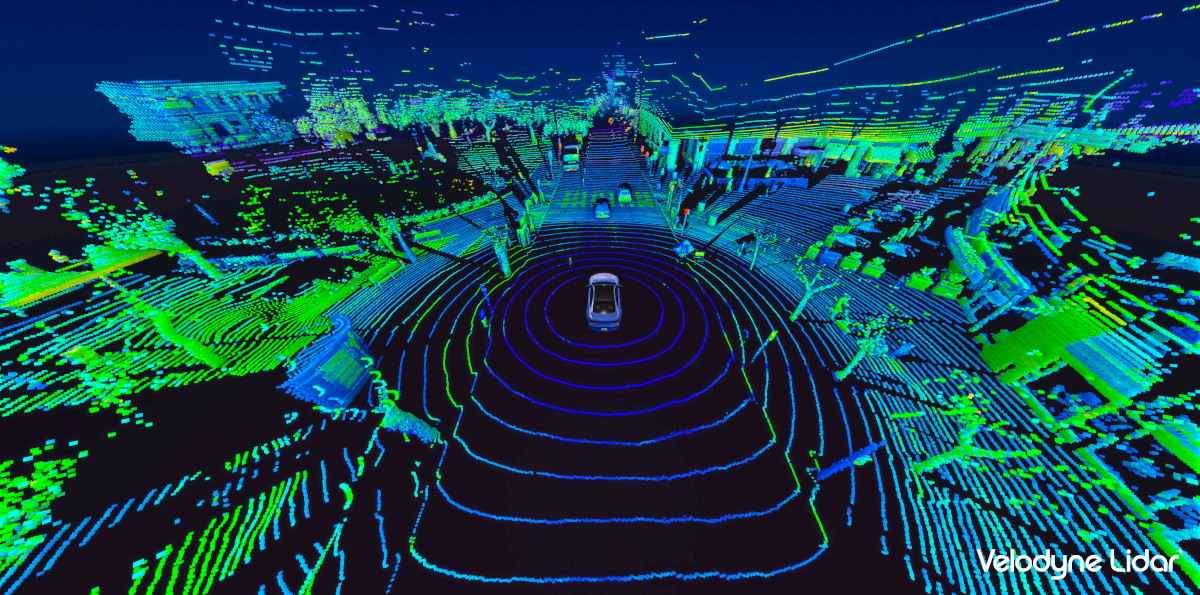
\includegraphics[width=\textwidth]{images/velodyne_pointcloud.jpg}\\
        \tiny{Source: Velodyne\footnotemark[1]}
    \end{column}
    \begin{column}{.5\textwidth}
        \footnotesize
        Only very recently has lidar been introduced in production vehicles, but it has
        been a core sensor of autonomous driving research since the DARPA challenges.
        \vspace{0.2cm}
        \begin{columns}[T]
            \begin{column}{0.4\textwidth}
                \footnotesize
                Capabilities:
                \begin{itemize}
                    \item Dynamic and static object detection
                    \item Road boundary and curb detection
                    \item Lane detection
                \end{itemize}
            \end{column}
            \begin{column}{0.6\textwidth}
                \footnotesize
                Important properties:
                \begin{itemize}
                    \item High resolution
                    \item Large field of view
                    \item Measure intensity
                    \item Poor weather robustness
                    \item No velocity measurement
                \end{itemize}
            \end{column}
        \end{columns}
    \end{column}
\end{columns}
\footnotetext[1]{\tiny{\url{https://velodynelidar.com/media-kit/}}}
\end{frame}

\subsection{Perception}

\begin{frame}
\frametitle{Perception}
\framesubtitle{Object Detection and Tracking}
\begin{columns}[T]
    \begin{column}{.45\textwidth}
        \centering
        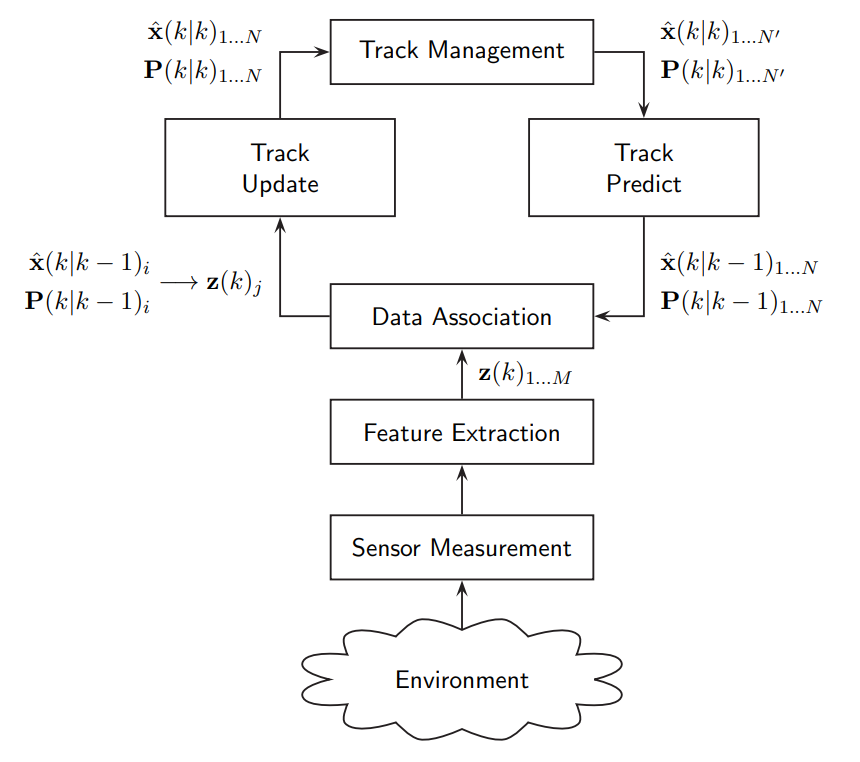
\includegraphics[width=0.75\textwidth]{images/aeberhard_tracking.png}\\
        \tiny{Common tracking architecture \cite{AeberhardDissertation}}\\
        \vspace{0.25cm}
        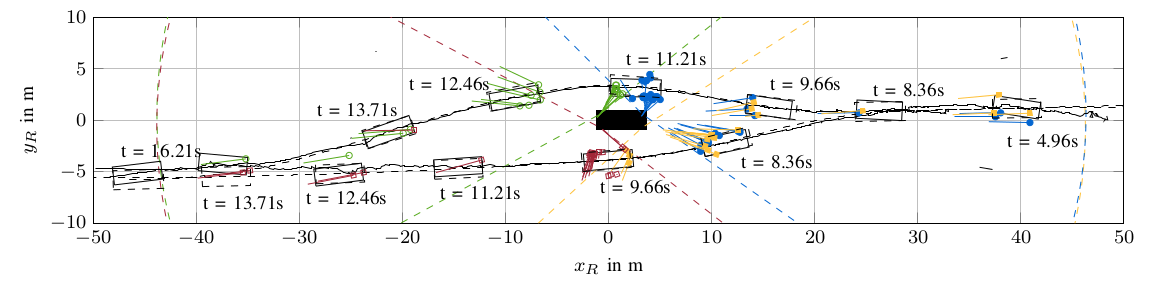
\includegraphics[width=\textwidth]{images/scheel_radar_tracking.png}\\
        \tiny{Tracking two objects with radar measurements \cite{Scheel2019}}
    \end{column}
    \begin{column}{.55\textwidth}
        Detection of dynamic objects is one of the central components in an
        AV system, with a very long history.
        \begin{itemize}
            \item Core algorithm is the Kalman filter \cite{Kalman1960}
                (and many variations therefore of) to estimate an object's
                state over time
            \item Bounding boxes are the most common representation form
            \item Pre-processing algorithms usually detect objects in a single
                data frame (clustering, ML-based detection, etc.)
        \end{itemize}
    \end{column}
\end{columns}
\end{frame}

\begin{frame}
\frametitle{Perception}
\framesubtitle{Occupancy Grids}
\begin{columns}[]
    \begin{column}{.5\textwidth}
        \centering
        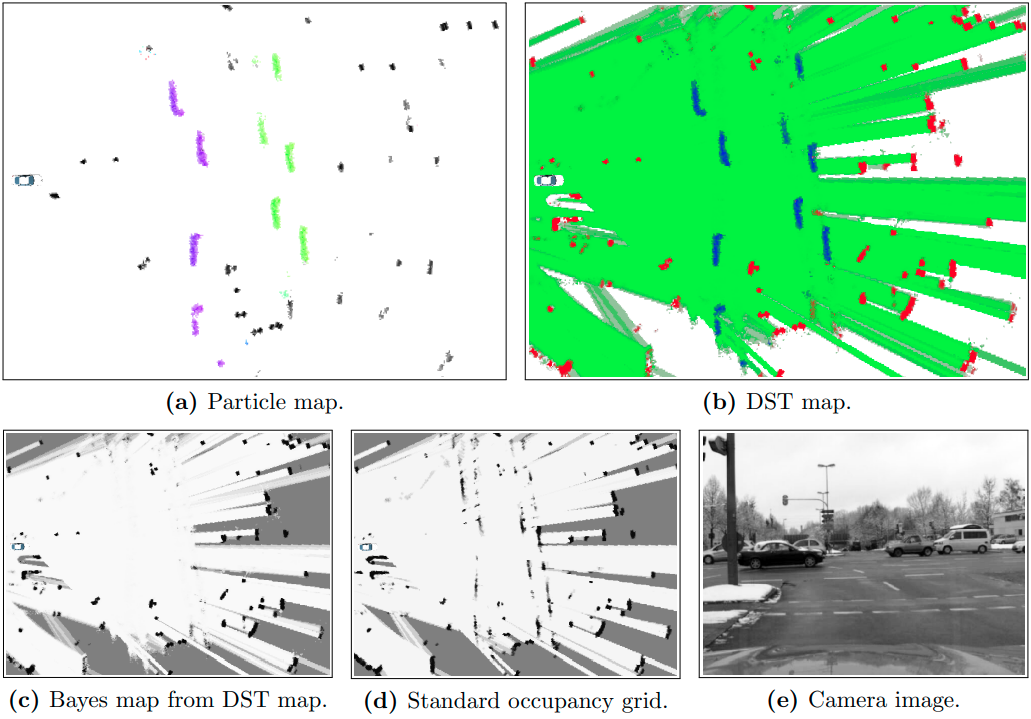
\includegraphics[width=\textwidth]{images/tanzmeister_dynamic_grids.png}\\
        \tiny{Dynamic occupancy grids \cite{TanzmeisterDissertation2016}}
    \end{column}
    \begin{column}{.5\textwidth}
        \footnotesize
        Occupancy grids have been a core algorithm in robotics since the
        mid-80s \cite{Moravec1985-ef} and have advanced ever since.
        \begin{itemize}
            \item Environment is rasterized into cells and a probability of
                occupancy is calculated
            \item Modern versions also calculate if a cell is dynamic or static
                or even the class (semantic)
            \item Free space (cells with no occupancy)
            \item Can be extended to include height information (elevation maps)
            \item Base environment representation which can be used by downstream
                component, e.g. object detection/tracking, localization, free space
                detection, etc.
        \end{itemize}
    \end{column}
\end{columns}
\end{frame}

\begin{frame}
\frametitle{Perception}
\framesubtitle{Lane / Road Detection}

\end{frame}

\begin{frame}
\frametitle{Perception}
\framesubtitle{Sensor Data Fusion}

\end{frame}

\subsection{Localization and Planning}

\begin{frame}
\frametitle{Localization}
Highly detailed maps for autonomous driving provide vital prior information
for navigating complex driving scenarios. Localization uses the sensor data
to localize the vehicle within such maps.\\
\vspace{0.25cm}
\centering
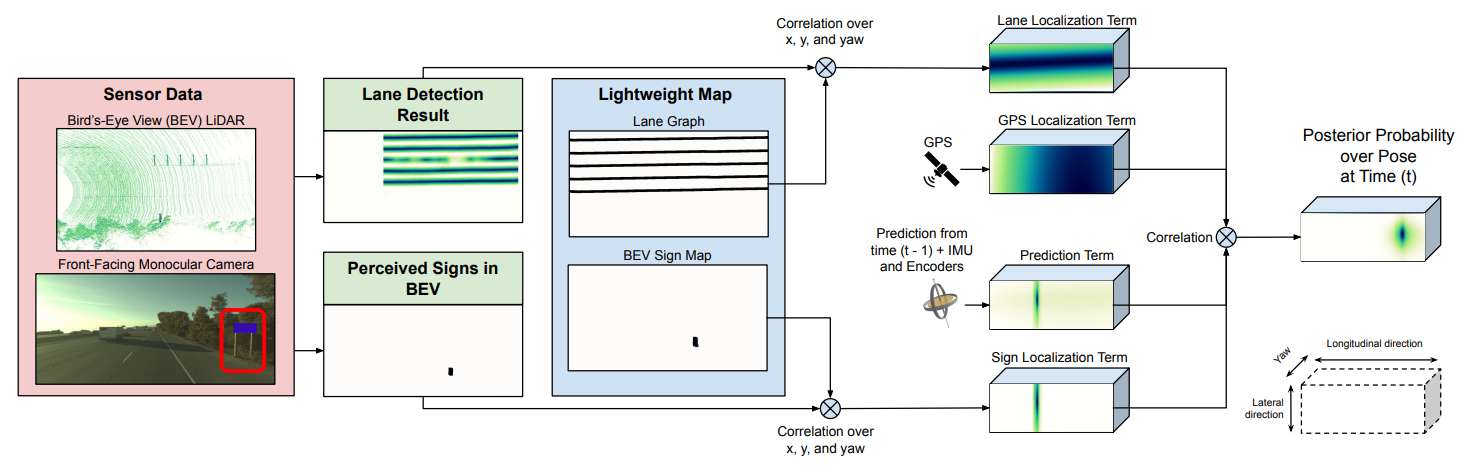
\includegraphics[width=\textwidth]{images/uber_sparse_localization.png}\\
\footnotesize{Localization on a sparse lane and traffic sign map on highways \cite{Ma2019}}
\end{frame}

\begin{frame}
\frametitle{Prediction}
Predicting the future trajectory of traffic is one of the core challenges in
advancing the performance of autonomous vehicles.\\
\vspace{0.25cm}
\centering
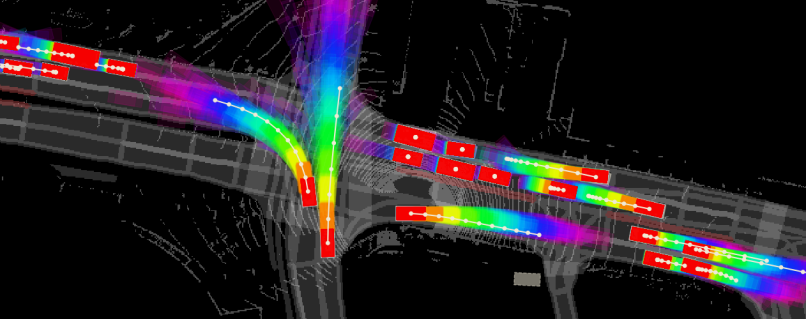
\includegraphics[width=0.8\textwidth]{images/uber_prediction.png}\\
\vspace{0.2cm}
\footnotesize{Heat map of future locations of traffic over time
      (white line is actual trajectory) \cite{Casas2020}}
\end{frame}

\begin{frame}
\frametitle{Motion Planning}
Based on the perception, localization and prediction input, motion planning
plans a safe trajectory for the vehicle to follow. Sampling-based and
optimization methods are the most common approaches.\\
\centering
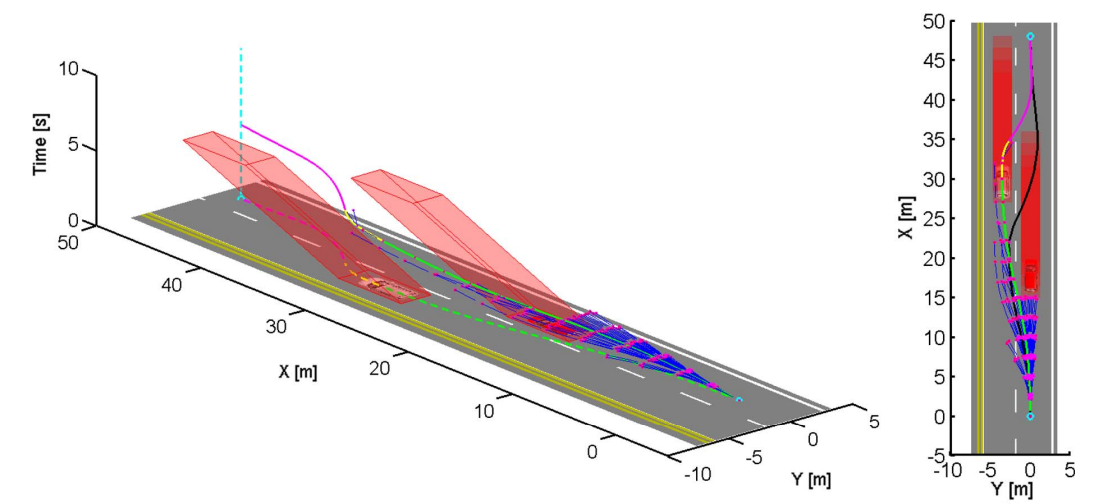
\includegraphics[width=0.8\textwidth]{images/ma_motionplanning.png}\\
\footnotesize{Motion planning in a highway scenario \cite{Ma2015}}
\end{frame}

\subsection{Machine Learning}

\begin{frame}
\frametitle{Machine Learning in Autonomous Driving}
Recent advances in machine learning, in particular deep neural networks, have
affected the algorithmic approach in almost all components in an AV stack.
\begin{columns}[]
    \begin{column}{0.4\textwidth}
        \begin{itemize}
            \item Algorithms are not designed, but models are rather learned
                from (labeled) data
            \item Performance of certain tasks, in particular with computer
                vision, have made major leaps forward
            \item Requires large amount of data
            \item Requires specialized hardware for efficient, real-time 
                processing
        \end{itemize}
    \end{column}
    \begin{column}{0.6\textwidth}
        \centering
        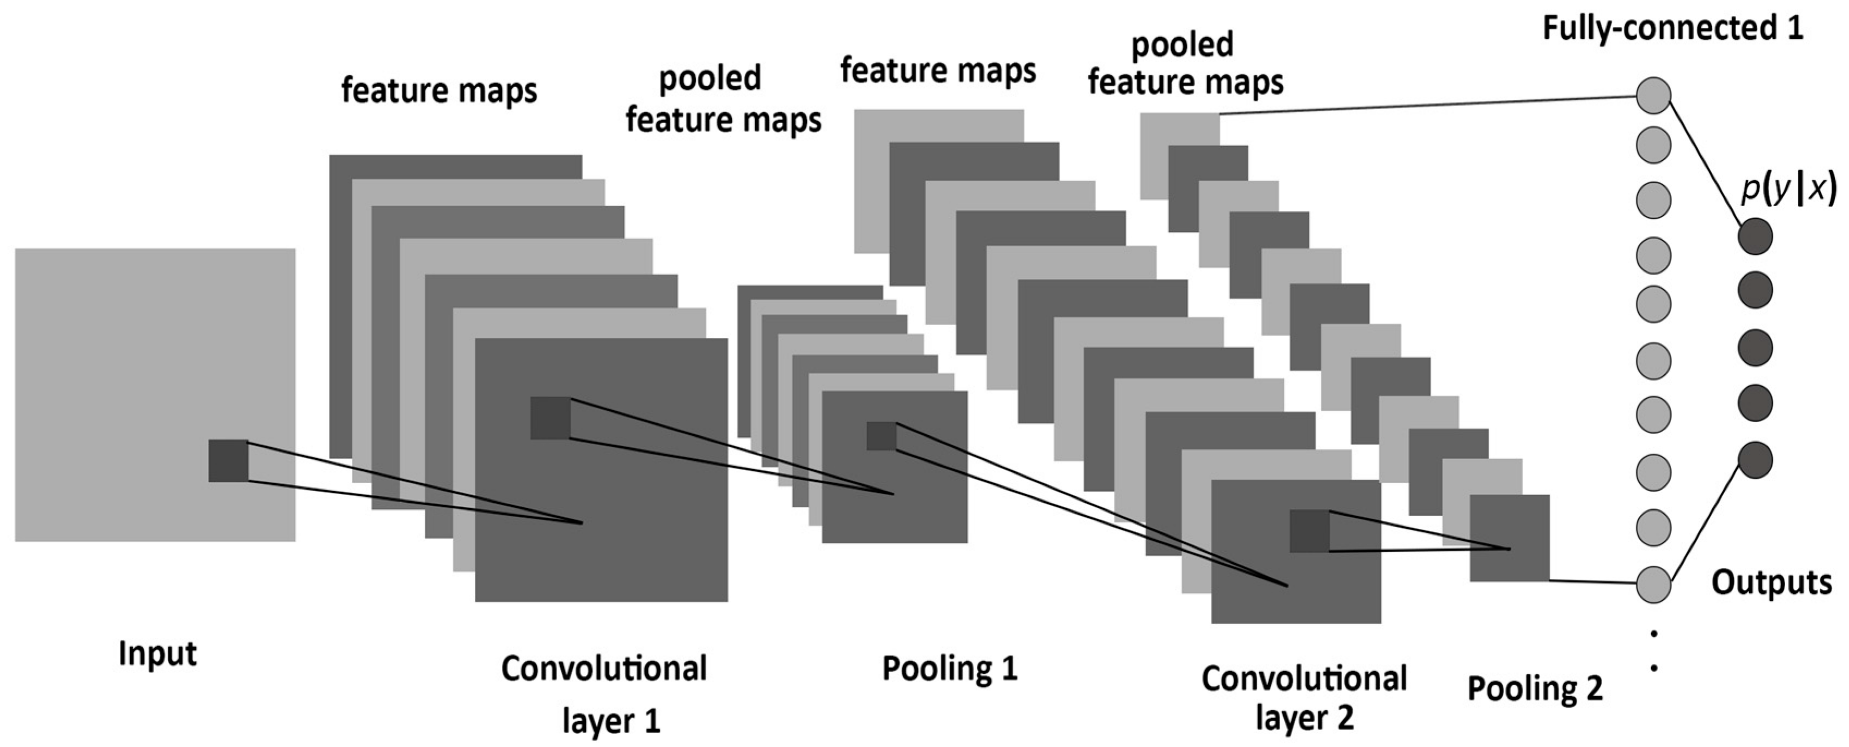
\includegraphics[width=\textwidth]{images/cnn_architecture.png}\\
        \footnotesize{Convolutional neural network architecture for image classification \cite{Albelwi2017}}
    \end{column}
\end{columns}
\end{frame}

\begin{frame}
\frametitle{Machine Learning in Autonomous Driving}
\framesubtitle{Examples for camera sensors}
\begin{columns}[]
    \begin{column}{0.6\textwidth}
        \centering
        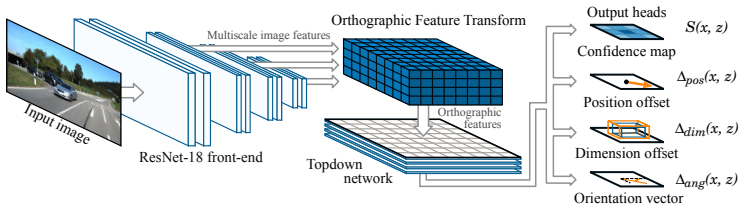
\includegraphics[width=\textwidth]{images/roddick_3d_camera_network.png}\\
        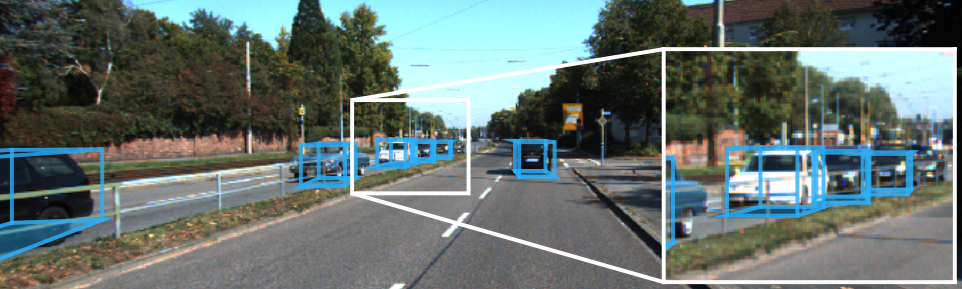
\includegraphics[width=\textwidth]{images/roddick_3d_camera_detections.png}\\
        \vspace{0.1cm}
        \footnotesize{3D camera object detection \cite{Roddick2019}}
    \end{column}
    \begin{column}{0.4\textwidth}
        \centering
        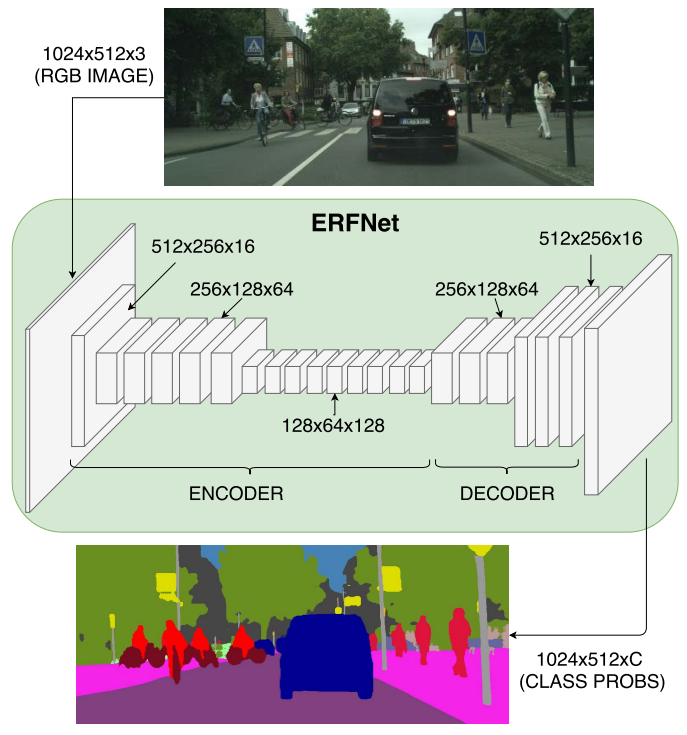
\includegraphics[width=0.9\textwidth]{images/erfnet_semantic_segmentation.png}\\
        \footnotesize{Semantic segmentation \cite{Romera2018}}
    \end{column}
\end{columns}
\end{frame}

\begin{frame}
\frametitle{Machine Learning in Autonomous Driving}
\framesubtitle{Examples for lidar sensors}
\centering
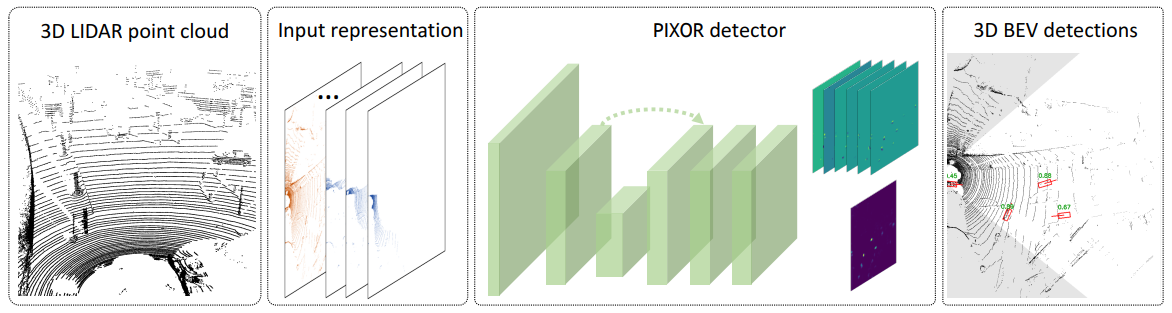
\includegraphics[width=\textwidth]{images/pixor_lidar_object_detection.png}\\
\footnotesize{3D lidar object detection \cite{Yang2018}}
\end{frame}

\begin{frame}
\frametitle{Machine Learning in Autonomous Driving}
\framesubtitle{Examples for lidar sensors}
\centering
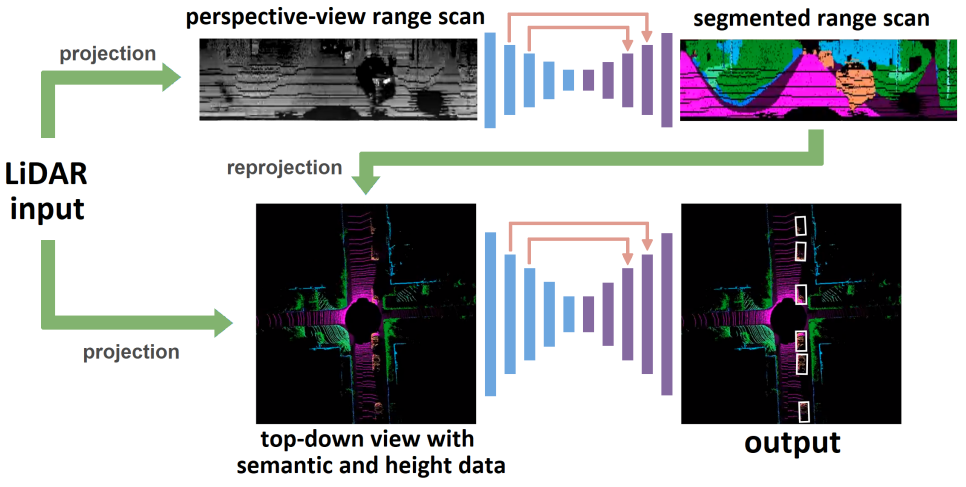
\includegraphics[width=0.8\textwidth]{images/nvidia_lidar_semantic_segmentation.png}\\
\vspace{0.2cm}
\footnotesize{Lidar semantic segmentation \cite{Chen2020}}
\end{frame}

\begin{frame}
\frametitle{Machine Learning in Autonomous Driving}
\framesubtitle{Examples for sensor data fusion}
Deep neural networks can take several sensors as input to realize a learned
approach to sensor data fusion.\\
\vspace{0.25cm}
\centering
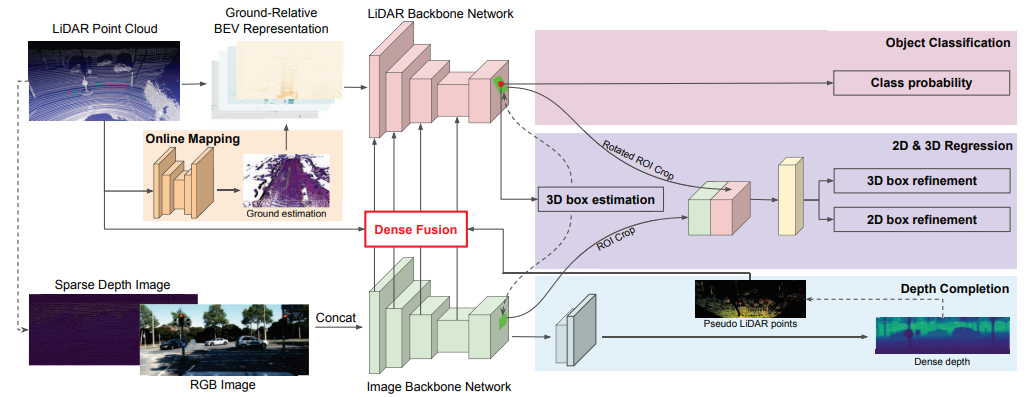
\includegraphics[width=0.9\textwidth]{images/uber_dnn_sensor_fusion.png}\\
\vspace{0.1cm}
\footnotesize{DNN with combined training of lidar and camera \cite{Liang2019}}
\end{frame}

\begin{frame}
\frametitle{Machine Learning in Autonomous Driving}
\framesubtitle{Example for planning components}
ChauffeurNet is an example of deep neural networks directly driving the vehicle
and learning the tasks of prediction and planning.\\
\begin{columns}[T]
    \begin{column}{0.4\textwidth}
        \centering
        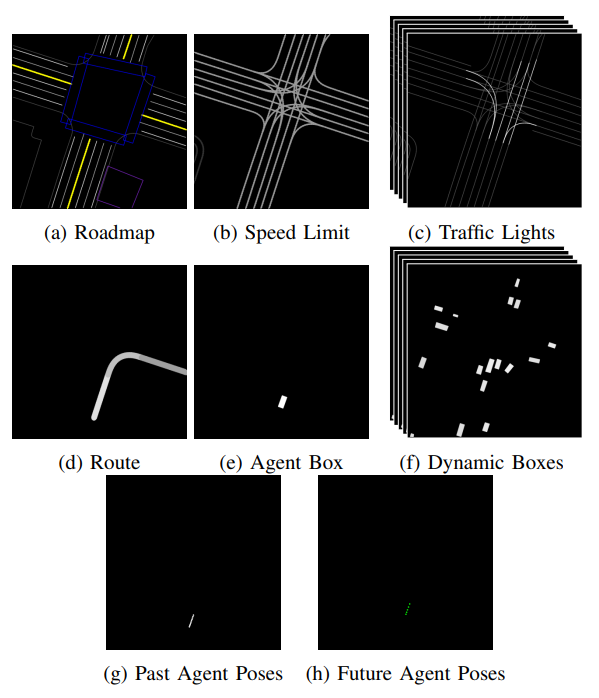
\includegraphics[width=0.7\textwidth]{images/waymo_chauffeurnet_inputs.png}\\
    \end{column}
    \begin{column}{0.6\textwidth}
        \centering
        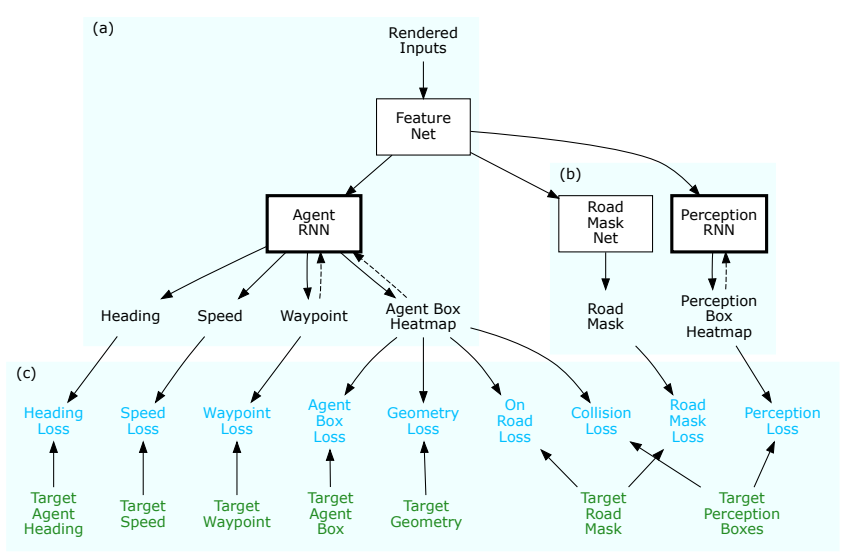
\includegraphics[width=0.8\textwidth]{images/waymo_chauffeurnet_network.png}\\
    \end{column}
\end{columns}
\vspace{0.2cm}
\centering
\footnotesize{ChauffeurNet input images and training architecture \cite{Bansal2019}}
\end{frame}

\subsection{Additional Topics}

\begin{frame}
\frametitle{Architecture for Safety}
A key challenge in autonomous driving is designing a functional architecture
which is robust to failures.

\begin{columns}[T]
    \begin{column}{0.35\textwidth}
        \centering
        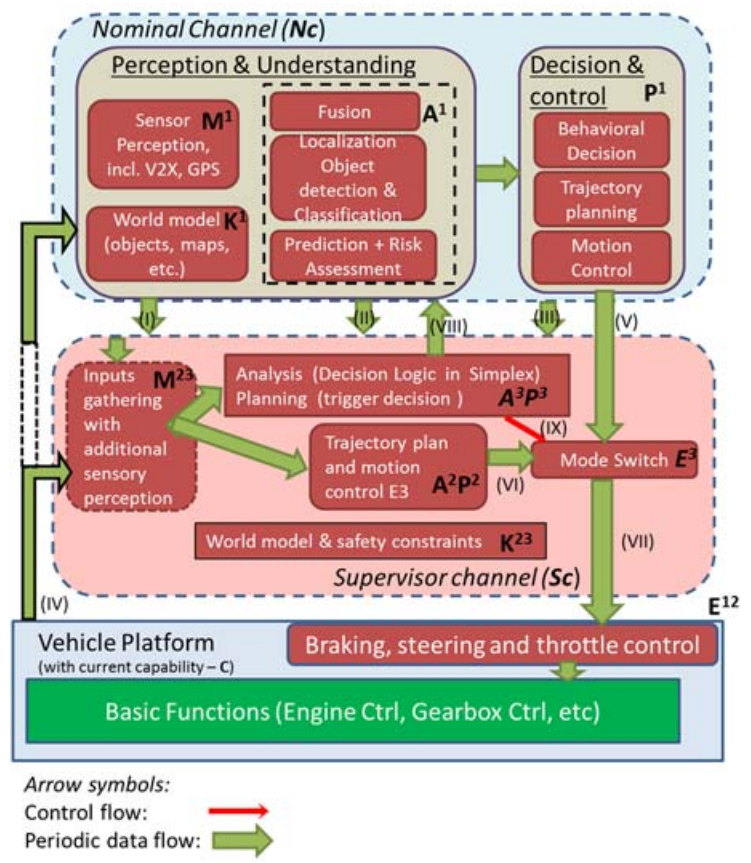
\includegraphics[width=0.95\textwidth]{images/redundant_architecture.png}\\
        \vspace{0.2cm}
        \tiny{Redundant supervisor channel \cite{Torngren2018}}
    \end{column}
    \begin{column}{0.65\textwidth}
        \begin{itemize}
            \item Some form of functional redundancy is required
            \item The redundant system is usually simpler and focuses only on
                safety goals, e.g. collision avoidance
            \item Overrides main system or applies constraints
        \end{itemize}
        \centering
        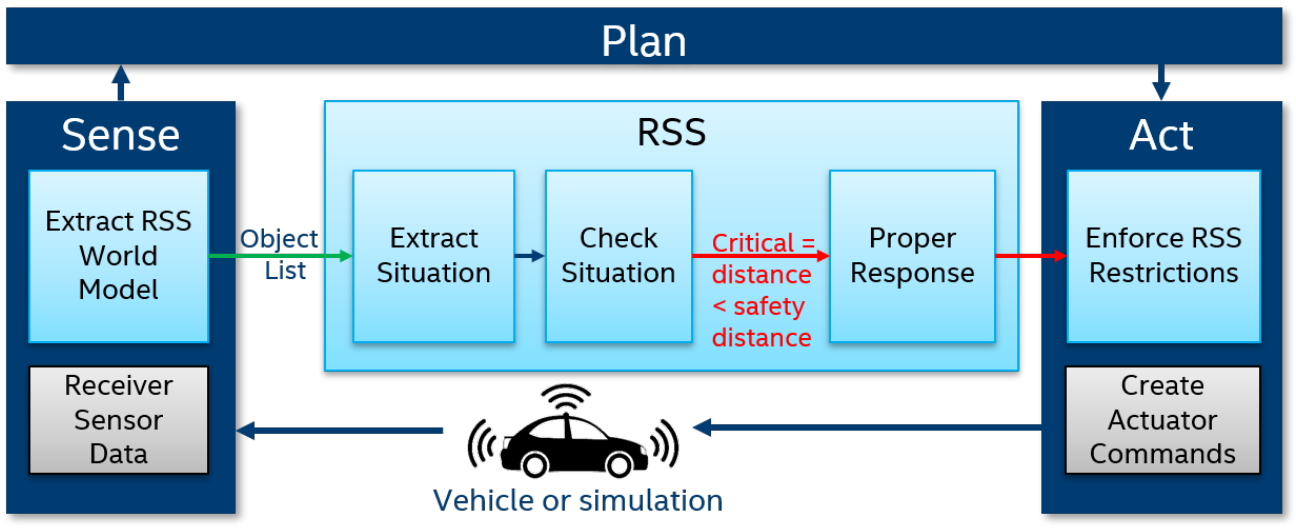
\includegraphics[width=0.75\textwidth]{images/intel_rss.png}\\
        \vspace{0.15cm}
        \tiny{Responsibility Sensitive Safety from Intel/MobilEye \cite{IntelRSS}}
    \end{column}
\end{columns}
\end{frame}

% \begin{frame}
% \frametitle{Datasets}

% \end{frame}

% \begin{frame}
% \frametitle{Books}

% \end{frame}